\section{Закон сохранения энергии}

\begin{ex}
\hspace{0pt} \\
\begin{minipage}{.65\textwidth}
(2004) В длинной теплоизолированной трубке между одинаковыми поршнями массы $m$ находится 1 моль одноатомного идеального газа при температуре $T_0$. 
В начальный момент скорости поршней направлены в одну сторону и равны $v$ и $3v$. До какой максимальной температуры нагреется газ? 
Поршни тепло не проводят, массой газа по сравнению с массой поршней пренебречь.
\end{minipage}
\begin{minipage}{.35\textwidth}
\centering
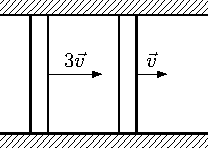
\includegraphics[width = 0.9 \textwidth]{0901LawOfConservationOfEnergyTwoPistons.jpg}
\end{minipage}
\begin{ans}
$T=T_0+2mv^2/3R$
\end{ans}
\end{ex}

%Черепанов
\begin{ex}
В длинной горизонтальной трубе могут скользить без трения два поршня, массы которых $m$ и $2m$. 
Между ними находится некоторое количество одноатомного газа при давлении $p$ и объеме $V$. 
В этот момент легкий поршень движется к тяжелому со скоростью $v_0$, тяжелый поршень покоится. 
Оцените максимальную скорость тяжелого поршня.
\begin{ans}
$v = v_0\left( 1 + \sqrt{1+9pV/2mv_0^2} \right)/3$
\end{ans}
\end{ex}

\begin{ex}
(2003) Внутри закрытого теплоизолированного цилиндра с идеальным газом находится легкоподвижный теплопроводящий поршень. 
При равновесии поршень делит цилиндр на две равные части и температура газа равна $T_0$. Поршень начали медленно перемещать. 
Найти температуру газа как функцию отношения $\eta$ объема большей части к объему меньшей части. Показатель адиабаты газа~$\gamma$.
\begin{ans}
$T=T_0 \left( (\eta + 1)^2/4 \eta \right)^{(\gamma-1)/2}$
\end{ans}
\end{ex}

\begin{ex}
\hspace{0pt} \\
\begin{minipage}{.65\textwidth}
Найдите КПД тепловой машины, цикл которой состоит из двух изохор и двух изобар, а рабочим телом является идеальный одноатомный газ. 
Середины нижней изобары и левой изохоры лежат на изотерме, соответствующей температуре $T_1$, 
а середины верхней изобары и правой изохоры -- на изотерме, соответствующей температуре~$T_2$.
\end{minipage}
\begin{minipage}{.35\textwidth}
\centering
\includestandalone{Pictures/0904LawOfConservationOfEnergyEfficiency}
\end{minipage}
\begin{ans}
$\eta = \frac{2(T_2-T_1)}{3T_1+5T_2}$
\end{ans}
\end{ex}

\begin{ex}
(2014) В вертикальном цилиндрическом сосуде с теплонепроницаемыми стенками под поршнем массы $m$~=~100~г находится 5 моль неона 
(молярная масса 20 г/моль). В начальный момент поршень закреплен. После того, как поршень освободили, объем газа увеличился в 2 раза. 
Определите конечную температуру газа, если его начальная температура равна $T_0$ = 300~К. Считайте, что над поршнем вакуум. 
Трением между поршнем и стенками сосуда отсутствует.
\begin{ans}
$T=2T_0/3 = 200$ К
\end{ans}
\end{ex}

\begin{ex}
(2015) B высоком теплоизолированном цилиндре под поршнем находится гелий. Над поршнем — вакуум. Поршню толчком сообщают скорость 2 м/с. На сколько выше или ниже начального положения окажется поршень после прихода системы в равновесие? Трением и теплообменом с внешней средой пренебречь.
\begin{ans}
$\Delta h = v_0^2 / 5g = 8$ см
\end{ans}
\end{ex}

\begin{ex}
(2016) B цилиндрическом сосуде с диэлектрическими стенками между металлическим основанием и металлическим поршнем находится двухтомный идеальный газ. Поршень и основание являются обкладками конденсатора, заряженного до напряжения $U$ и отключенного от источника питания, В равновесии расстояние между поршнем и основанием цилиндра равно $d$ (много меньше радиуса цилиндра) Площадь сечения сосуда равна $S$, слева от поршня - вакуум.
1) Определите отношение внутренней энергии газа и энергии электрического поля конденсатора. 2) Какое количество теплоты нужно сообщить газу для того, чтобы медленно увеличить расстояние между обкладками в 2 раза?
\begin{center}
\includestandalone{Pictures/GasInsideCapacitor}
\end{center}
\begin{ans}
1) $U/W=5/2$; 2) $Q=\frac{7\varepsilon_0 SU^2}{4d}$.
\end{ans}
\end{ex}

\begin{ex}
(2002) Чему равна работа 1 моля идеального газа в круговом процессе, показанном на рисунке? Температуры $T_1$ и $T_2$ известны.
\begin{center}
\includestandalone{Pictures/092002LawOfConservationOfEnergyProcess}
\end{center}
\begin{ans}
$A= R(T_2-T_1)-RT_1 \log T_2/T_1$
\end{ans}
\end{ex}

\begin{ex}
\hspace{0pt} \\
\begin{minipage}{.65\textwidth}
(2017) Идеальный одноатомный газ в количестве 0,1 моль находится под массивными поршнями в двух сообщающихся сосудах. Сосуды закрыты и откачаны, т.е. над поршнями вакуум. Массы поршней $m_1 = m_2 = 10$ кг, площади поперечного сечения поршней $S_1 = 10$ см\textsuperscript{2}, $S_2 = 20$ см\textsuperscript{2} B начальный момент времени первый поршень свободен, a второй — зафиксирован, поршни находятся на одинаковой высоте $h_1 = 80$ см. 1) Определите начальную температуру газа. 2) До какой температуры нагреется газ, если ему квазистатически сообщить тепло 100 Дж? 3) Определите температуру газа, которая установится, если в начальный момент времени сосуды теплоизолировать и освободить второй поршень. Трение отсутствует. Сосуды высокие, объемом очень тонкой перегородки, соединяющей сосуды, пренебречь. Ускорение свободного падения $g = 10$ м/c\textsuperscript{2}.
\end{minipage}
\begin{minipage}{.35\textwidth}
\centering
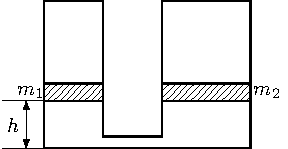
\includegraphics[width = 0.9 \textwidth]{TwoVessels.png}
\end{minipage}
\begin{ans}
1) $T_0 = m_1gh(1+S_2/S_1)/(\nu R) = 289$ К;
2) $T_2 = T_0 + 2Q/(5\nu R) = 337$ К; 
3) $T_3 = \frac{2}{5\nu R}(m_1 gh + m_2 gh)+ \frac{3}{5}T_0 = 250$ К.
\end{ans}
\end{ex}

\section{Теплоемкость}

\begin{ex}
(1998) Имеется идеальный газ, теплоемкость которого при постоянном объеме равна $C_V$. 
Найдите молярную теплоемкость этого газа как функцию объема, если давление газа меняется по закону $p=p_0~e^{\alpha V}$ ($p_0$ и $\alpha$ известны).
\begin{ans}
$C = C_V + R/(1+\alpha)$
\end{ans}
\end{ex}

%Черепанов
\begin{ex}
Для идеального газа с заданным показателем адиабаты $\gamma$ найдите уравнение процесса (в координатах $V$, $T$), при котором теплоемкость зависит от температуры по закону $C=\alpha T^2$.
\begin{ans}
$ V T^{1/(\gamma - 1)} = C e^{\alpha T^2 / 2R}$
\end{ans}
\end{ex}

\begin{ex}
\hspace{0pt} \\
\begin{minipage}{.65\textwidth}
(2005) В расположенном горизонтально цилиндре слева от закрепленного поршня находится один моль идеального газа, в правой части цилиндра - вакуум. Цилиндр теплоизолирован от окружающей среды, а пружина, расположенная между поршнем и стенкой, находится первоначально в недеформированном состоянии. Поршень освобождают, и после установления равновесия объем, занимаемый газом, увеличивается в $\alpha$ раз. Как изменились при этом температура и давление газа? Теплоемкостями цилиндра, поршня и пружины пренебречь. Найти теплоемкость газа.
\end{minipage}
\begin{minipage}{.35\textwidth}
\centering
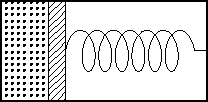
\includegraphics[width = 0.9 \textwidth]{092005HeatCapacityCylinder.jpg}
\end{minipage}
\begin{ans}
$T_2/T_1 = (\alpha i)/(\alpha (1+i) - 1)$, $p_2/p_1 = i/(\alpha (1+i) - 1)$
\end{ans}
\end{ex}

\begin{ex}
(2001) Вычислить молярную теплоемкость $C(V)$ идеального газа, совершающего процесс, показанный на рисунке. Показатель адиабаты $\gamma$ считать известным.
\begin{center}
\includestandalone{Pictures/082001GasLawsProcess}
\end{center}
\begin{ans}
$C(V) = R/(\gamma-1)+R(V_0-2V)/(V_0-2V)$
\end{ans}
\end{ex}